\documentclass[xetex,mathserif,serif,aspectratio=169]{beamer}

\usepackage{xltxtra}
\usepackage{color}
\usepackage{url}
\usepackage{listings}
\usepackage{fontspec}
\usepackage{geometry}
\usepackage{lastpage}
\usepackage{fancyhdr}
\usepackage{amsmath}
\usepackage{amsthm}
\usepackage{amssymb}
\usepackage{blkarray}
\usepackage{multicol}
\usepackage{relsize}
\usepackage{listings}
\usepackage{xunicode}
\usepackage{xltxtra}
\usepackage{color}
\usepackage{url}
\usefonttheme[onlymath]{serif}

\definecolor{solarized@base03}{HTML}{002B36}
\definecolor{solarized@base02}{HTML}{073642}
\definecolor{solarized@base01}{HTML}{586e75}
\definecolor{solarized@base00}{HTML}{657b83}
\definecolor{solarized@base0}{HTML}{839496}
\definecolor{solarized@base1}{HTML}{93a1a1}
\definecolor{solarized@base2}{HTML}{EEE8D5}
\definecolor{solarized@base3}{HTML}{FDF6E3}
\definecolor{solarized@yellow}{HTML}{B58900}
\definecolor{solarized@orange}{HTML}{CB4B16}
\definecolor{solarized@red}{HTML}{DC322F}
\definecolor{solarized@magenta}{HTML}{D33682}
\definecolor{solarized@violet}{HTML}{6C71C4}
\definecolor{solarized@blue}{HTML}{268BD2}
\definecolor{solarized@cyan}{HTML}{2AA198}
\definecolor{solarized@green}{HTML}{859900}
\definecolor{yaleblue}{HTML}{0E4C92}

\newcommand{\yellow}[1]{\textcolor{solarized@yellow}{#1}}
\newcommand{\orange}[1]{\textcolor{solarized@orange}{#1}}
\newcommand{\red}[1]{\textcolor{solarized@red}{#1}}
\newcommand{\magenta}[1]{\textcolor{solarized@magenta}{#1}}
\newcommand{\violet}[1]{\textcolor{solarized@violet}{#1}}
\newcommand{\blue}[1]{\textcolor{solarized@blue}{#1}}
\newcommand{\cyan}[1]{\textcolor{solarized@cyan}{#1}}
\newcommand{\green}[1]{\textcolor{solarized@green}{#1}}
\newcommand{\yblue}[1]{\textcolor{yaleblue}{#1}}
\newcommand{\base}[1]{\textcolor{solarized@base01}{#1}}


\defaultfontfeatures{Mapping=tex-text}
\hypersetup{pdfstartview={FitH}}

\newcommand{\old}[1]{\fontspec[Alternate=1,Ligatures={Common}]{Hoefler Text}\fontsize{18pt}{30pt}\selectfont #1}%
\newcommand{\oldA}[1]{\fontspec[Alternate=1,Ligatures={Common, Rare}]{Hoefler Text}\fontsize{12pt}{15pt}\selectfont #1}%
\newcommand{\oldB}[1]{\fontspec[Ligatures={Common}]{Didot}\fontsize{12pt}{15pt}\color{solarized@base02}\selectfont #1}%
\newcommand{\tfont}[1]{\fontspec[Alternate=1,Ligatures={Common}]{Hoefler Text}\fontsize{12pt}{20pt}\selectfont #1}%
\newcommand{\dfont}[1]{\fontspec[Ligatures={Common}]{Didot}\fontsize{12pt}{12pt}\selectfont #1}%

\setbeamerfont{title}{family=\old}
\setbeamerfont{author}{family=\tfont}%
\setbeamerfont{frametitle}{family=\oldA}
\setbeamerfont{date}{family=\dfont}

\setbeamertemplate{navigation symbols}{}
\setbeamertemplate{footline}[text line]{%
  \parbox{0.99\linewidth}{
    \normalsize\vspace*{-24pt}\hfill{\color{solarized@base00}\insertframenumber/\inserttotalframenumber}
  }
}


\setlength{\parindent}{0pt}
\setlength{\parskip}{12pt}

\setbeamercolor{structure}{bg=solarized@base3, fg=solarized@base02}
\setbeamercolor{titlelike}{fg=solarized@cyan}
\setbeamercolor{title}{fg=solarized@blue}
\setbeamercolor{subtitle}{fg=solarized@magenta}
\setbeamercolor{alerted text}{fg=orange}
\setbeamercolor{itemize}{fg=solarized@base02}
\setbeamercolor{background canvas}{bg=solarized@base3}
\setbeamercolor{enumerate subitem}{fg=solarized@base02}

\newcommand{\minimize}{\mathop{\mathrm{minimize}}}
\newcommand{\argmin}{\mathop{\mathrm{arg\,min}}}
\newcommand{\argmax}{\mathop{\mathrm{arg\,max}}}
\newcommand{\st}{\mathop{\mathrm{subject\,\,to}}}



\begin{document}

%%%%%%%%%%%%%%%%%%%%%%%%%%%%%%%%%%%%%%%%%%%%%%%%%%%
\begin{frame}[fragile] \frametitle{} \oldB \small

\vfill

{\fontsize{0.7cm}{0cm}\selectfont Lecture 04 \\\vspace{0.2cm} Least squares and classification}\\\vspace{0.5cm}
27 January 2016

\vspace{2cm}

\begin{minipage}{0.6\textwidth}
Taylor B. Arnold \\
Yale Statistics \\
STAT 365/665
\end{minipage}
\hfill
\begin{minipage}{0.3\textwidth}\raggedleft

\includegraphics[scale=0.3]{../yale-logo.png}
\end{minipage}%

\end{frame}

%%%%%%%%%%%%%%%%%%%%%%%%%%%%%%%%%%%%%%%%%%%%%%%%%%%
\begin{frame}[fragile] \frametitle{} \oldB \small

\begin{itemize}
\item Problem set notes:
\begin{itemize}
\item brute force okay for implementation question
\item can use other libraries in the prediction and data analysis questions
\item consider \textbf{FNN} (R) or or \textbf{sklearn.neighbors} (Python)
\end{itemize}
\item Office hours (more possibly to come):
\begin{itemize}
\item Taylor Arnold -- Mondays, 13:00 - 14:15, HH 24, Office 206 (by appointment)
\item Yu Lu -- Tuesdays, 10:00-12:00, HH 24, Library
\item Jason Klusowski -- Thursdays, 19:00-20:30, HH 24
\end{itemize}
\end{itemize}

\end{frame}

%%%%%%%%%%%%%%%%%%%%%%%%%%%%%%%%%%%%%%%%%%%%%%%%%%%
\begin{frame}[fragile] \frametitle{} \oldB \small

\begin{center}
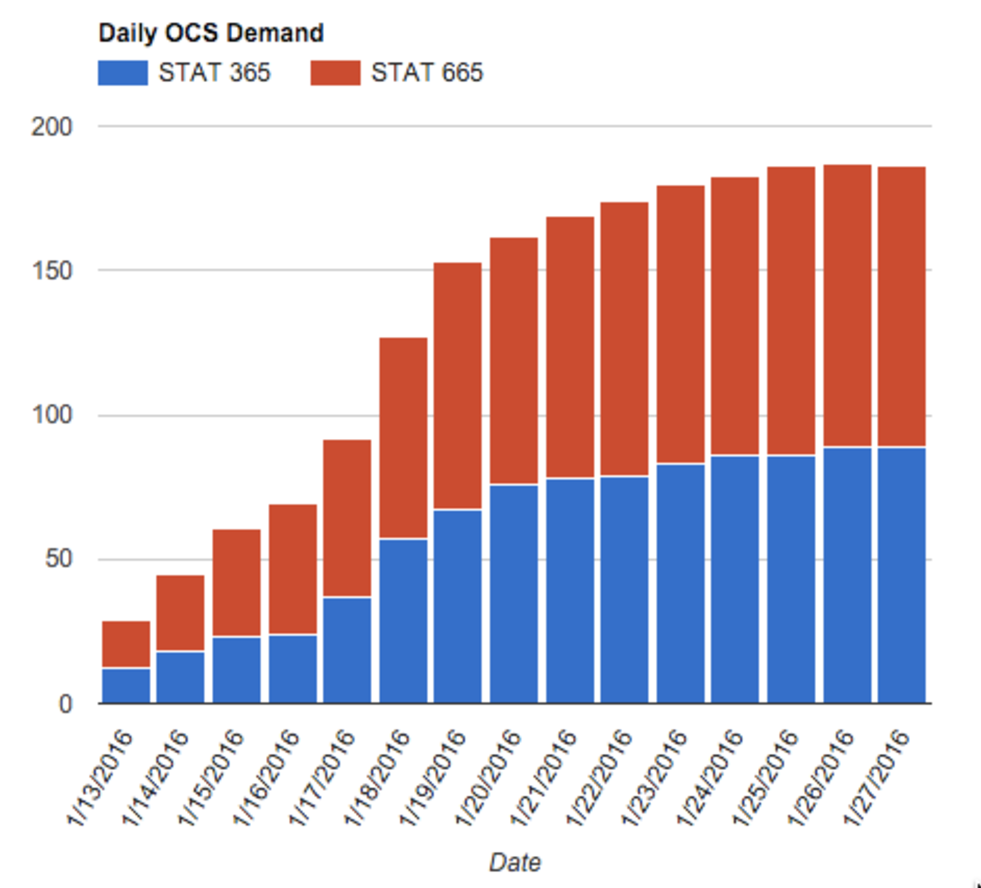
\includegraphics[width=0.7\textwidth]{img/stat665.pdf}
\end{center}

\end{frame}

%%%%%%%%%%%%%%%%%%%%%%%%%%%%%%%%%%%%%%%%%%%%%%%%%%%
\begin{frame}[fragile] \frametitle{} \oldB \small

\textbf{\yblue{Ordinary least squares}}

The multivariate linear regression model is given by:
\begin{align*}
y_i &= x_{1,i} \beta_1 + x_{2,i} \beta_2 + \cdots + x_{1,p} \beta_p + \epsilon_i
\end{align*}

\end{frame}


%%%%%%%%%%%%%%%%%%%%%%%%%%%%%%%%%%%%%%%%%%%%%%%%%%%
\begin{frame}[fragile] \frametitle{} \oldB \small

A sample can be re-written in terms of the vector $x_i$
(the vector of covariates for a single observation):
\begin{align*}
y_i &= x_{i}^t \beta + \epsilon_i
\end{align*}

\end{frame}

%%%%%%%%%%%%%%%%%%%%%%%%%%%%%%%%%%%%%%%%%%%%%%%%%%%
\begin{frame}[fragile] \frametitle{} \oldB \small

In matrix notation, we can write the linear model simultaneously
for all observations:
\begin{align*}
\left(\begin{array}{c}y_1\\ y_2\\ \vdots\\ y_n\end{array}\right) &=
  \left(\begin{array}{cccc}x_{1,1}&x_{2,1}&\cdots&x_{p,1}\\
                           x_{1,2}&\ddots&&x_{p,2}\\
                           \vdots&&\ddots&\vdots\\
                           x_{1,n}&x_{2,n}&\cdots&x_{p,n}\\\end{array}\right)
  \left(\begin{array}{c}\beta_1\\ \beta_2\\ \vdots\\ \beta_p\end{array}\right) +
  \left(\begin{array}{c}\epsilon_1\\ \epsilon_2\\ \vdots\\ \epsilon_n\end{array}\right)
\end{align*}
\pause Which can be compactly written as:
\begin{align*}
y &= X \beta + \epsilon
\end{align*}

\end{frame}

%%%%%%%%%%%%%%%%%%%%%%%%%%%%%%%%%%%%%%%%%%%%%%%%%%%
\begin{frame}[fragile] \frametitle{} \oldB \small

For reference, note the following equation
\begin{align*}
y &= X \beta + \epsilon
\end{align*}
Yields these dimensions:
\begin{align*}
y &\in \mathbb{R}^n \\
X &\in \mathbb{R}^{n \times p} \\
\beta &\in \mathbb{R}^p \\
\epsilon &\in \mathbb{R}^n \\
\end{align*}

\end{frame}

%%%%%%%%%%%%%%%%%%%%%%%%%%%%%%%%%%%%%%%%%%%%%%%%%%%
\begin{frame}[fragile] \frametitle{} \oldB \small

{\bf Least squares}

To estimate the least squares solution, which is again the
MLE for independent normal errors, we see that:
\begin{align*}
\widehat{\beta} \in \argmin_{b \in \mathbb{R}^p} \left\{ ||y - X b ||_2^2 \right\}
\end{align*}

\end{frame}

%%%%%%%%%%%%%%%%%%%%%%%%%%%%%%%%%%%%%%%%%%%%%%%%%%%
\begin{frame}[fragile] \frametitle{} \oldB \small

It will be helpful to re-write the sum of squares as:
\begin{eqnarray*}
||y - X \beta ||_2^2 &=& (y - X\beta)^t (y - X\beta) \\ \pause
&=& (y^t - \beta^t X^t) (y - X\beta) \\ \pause
&=& y^ty - y^t X\beta - \beta^t X^t y + \beta^t X^t X\beta \\ \pause
&=& y^ty - 2 y^t X\beta + \beta^t X^t X\beta
\end{eqnarray*}

\end{frame}

%%%%%%%%%%%%%%%%%%%%%%%%%%%%%%%%%%%%%%%%%%%%%%%%%%%
\begin{frame}[fragile] \frametitle{} \oldB \small

{\bf Normal Equations}

In order to find the minimum of the sum of squares, we take the gradient
with respect to $\beta$ and set it equal to zero.

Recall that, for a vector $a$ and symmetric matrix $A$ :
\begin{align*}
\nabla_\beta a^t \beta = a \\
\nabla_\beta \beta^t A \beta = 2 A \beta
\end{align*}
\pause This gives the gradient of the sum of squares as:
\begin{align*}
\nabla_\beta ||y - X \beta ||_2^2 &= \nabla_\beta \left(y^t y - {\color{solarized@blue} 2 y^t X\beta} + {\color{solarized@magenta} \beta^t X^t X\beta} \right)\\
&= {\color{solarized@magenta}2 X^t X \beta} - {\color{solarized@blue} 2 X^t y}
\end{align*}

\end{frame}

%%%%%%%%%%%%%%%%%%%%%%%%%%%%%%%%%%%%%%%%%%%%%%%%%%%
\begin{frame}[fragile] \frametitle{} \oldB \small

Setting this equal to zero gives a set of $p$ equations called
the normal equations:
\begin{align*}
X^t X \widehat{\beta} &= X^t y
\end{align*}

\end{frame}

%%%%%%%%%%%%%%%%%%%%%%%%%%%%%%%%%%%%%%%%%%%%%%%%%%%
\begin{frame}[fragile] \frametitle{} \oldB \small

{\bf Maximum or Minimum?}

To determine whether the normal equations give a local minimum, maximum, or
saddle point, we can calculate the Hessian matrix.
\pause This is a $p \times p$ matrix giving every combination of the
second partial derivatives:
\begin{align*}
H f(\beta) &=
  \left(\begin{array}{cccc}\frac{\partial^2f}{\partial \beta_1 \partial \beta_1}&\frac{\partial^2f}{\partial \beta_1 \partial \beta_2}&\cdots&\frac{\partial^2f}{\partial \beta_1 \partial \beta_p}\\
                           \frac{\partial^2f}{\partial \beta_2 \partial \beta_1}&\ddots&&\frac{\partial^2f}{\partial \beta_2 \partial \beta_p}\\
                           \vdots&&\ddots&\vdots\\
                           \frac{\partial^2f}{\partial \beta_p \partial \beta_1}&\frac{\partial^2f}{\partial \beta_p \partial \beta_2}&\cdots&\frac{\partial^2f}{\partial \beta_p \partial \beta_p}\\\end{array}\right)
\end{align*}
If the Hessian is positive definite ($x^t H x \geq 0$) at a critical point,
then the critical point is a local minimum.

\end{frame}

%%%%%%%%%%%%%%%%%%%%%%%%%%%%%%%%%%%%%%%%%%%%%%%%%%%
\begin{frame}[fragile] \frametitle{} \oldB \small

Looking at the gradient of the sum of squares:
\begin{align*}
\nabla_\beta ||y - X \beta ||_2^2 &= 2 X^t X \beta - 2 X^t y
\end{align*}
\pause We can see that the Hessian is simply:
\begin{align*}
H_\beta ||y - X \beta ||_2^2 &= 2 X^t X
\end{align*}
\pause Why is this positive definite? \pause
\begin{align*}
v^t \left(2 X^tX \right) v &= 2 \left( v^t X^t X v\right) \\
&= 2 || X v ||_2^2 \\
&\geq 0
\end{align*}

\end{frame}

%%%%%%%%%%%%%%%%%%%%%%%%%%%%%%%%%%%%%%%%%%%%%%%%%%%
\begin{frame}[fragile] \frametitle{} \oldB \small

Back to the normal equations themselves, notice that if the
matrix $X^t X$ is invertible, we can `solve' the normal
equations as:
\begin{align*}
X^t X \widehat{\beta} &= X^t y \\
\widehat{\beta} &= (X^t X)^{-1} X^t y
\end{align*}
\pause This is not a good way to solve the normal equations
numerically, but is a useful theoretical form.

\end{frame}

%%%%%%%%%%%%%%%%%%%%%%%%%%%%%%%%%%%%%%%%%%%%%%%%%%%
\begin{frame}[fragile] \frametitle{} \oldB \small

\textbf{\yblue{Ridge regression}}

The ridge regression estimator is the solution to the following
modified least squares optimization problem for some value of $\lambda > 0$.
\begin{align*}
\widehat{\beta}_{ridge} &= \argmin_b \left\{ || y - Xb ||_2^2 + \lambda || b ||_2^2 \right\}
\end{align*}

\end{frame}

%%%%%%%%%%%%%%%%%%%%%%%%%%%%%%%%%%%%%%%%%%%%%%%%%%%
\begin{frame}[fragile] \frametitle{} \oldB \small

Why the ridge penalty?
\begin{enumerate}
\item The equation shrinks the coefficients towards zero, adding some bias but
reducing the variance of the estimator. \pause
\item Using the $\ell_2$-norm keeps the equation rotationally invariant. \pause
\item Ridge regression has an analytical solution.
\end{enumerate}

\end{frame}

%%%%%%%%%%%%%%%%%%%%%%%%%%%%%%%%%%%%%%%%%%%%%%%%%%%
\begin{frame}[fragile] \frametitle{} \oldB \small

To see this write the criterion as a matrix equation:
\begin{align*}
(y - Xb)^t (y - Xb)  + \lambda b^t b
&= y^t y + b^t X^t X b - 2 y^t X b + \lambda b^t b \\
\end{align*}
\pause And take its derivative:
\begin{align*}
\frac{\partial}{\partial \beta} \left( y^t y + b^t X^t X b - 2 y^t X b + \lambda b^t b \right)
&= 2 X^t X b - 2 X^t y + 2 \lambda b
\end{align*}

\end{frame}

%%%%%%%%%%%%%%%%%%%%%%%%%%%%%%%%%%%%%%%%%%%%%%%%%%%
\begin{frame}[fragile] \frametitle{} \oldB \small

Setting this to zero yields
\begin{align*}
2 X^t X \widehat{\beta} + 2 \lambda \widehat{\beta} &= 2 X^t y \\
(X^t X + I_p \lambda) \widehat{\beta} &=  X^t y \\
\widehat{\beta} &= (X^t X + I_p \lambda)^{-1} \cdot X^t y \\
\end{align*}
\pause This is a useful analytical form, though as with least
squares we would generally not invert the matrix directly but
instead use a stable matrix decomposition.

\end{frame}


%%%%%%%%%%%%%%%%%%%%%%%%%%%%%%%%%%%%%%%%%%%%%%%%%%%
\begin{frame}[fragile] \frametitle{} \oldB \small

\textbf{\yblue{Computational issues}}

How can we estimate the regression vector using a technique
such as ordinary least squares
\begin{align*}
\widehat{\beta}_{ols} &= \argmin_b \left\{ \sum_{i=1}^n (y_i - x_i^t b)^2 \right\},
\end{align*}
When we have a dataset size grows larger than the available memory?

\end{frame}

%%%%%%%%%%%%%%%%%%%%%%%%%%%%%%%%%%%%%%%%%%%%%%%%%%%
\begin{frame}[fragile] \frametitle{} \oldB \small

At first glance this seems computationally very difficult
as we are trying to minimize a summation with one component
per observation.

However, recall that the ordinary least squares solution
can be computed by:
\begin{align*}
\widehat{\beta}_{ols} &= (X^t X)^{-1} X^t y.
\end{align*}

\end{frame}

%%%%%%%%%%%%%%%%%%%%%%%%%%%%%%%%%%%%%%%%%%%%%%%%%%%
\begin{frame}[fragile] \frametitle{} \oldB \small

Now, assume that the data matrix $X$ is broken by rows into
$K$ different chunks:
\begin{align*}
X &= \left( \begin{array}{c} X_{B_1} \\ X_{B_2} \\ \vdots \\ X_{B_K} \end{array} \right)
\end{align*}
\pause The Gram matrix $X^tX$ can then be computed by summing up the
Gram matrices of the individual chunks:
\begin{align*}
X^t X &= \sum_{i=1}^K X_{B_i}^t X_{B_i}.
\end{align*}

\end{frame}

%%%%%%%%%%%%%%%%%%%%%%%%%%%%%%%%%%%%%%%%%%%%%%%%%%%
\begin{frame}[fragile] \frametitle{} \oldB \small

If the vector $y$ is broken in to the same set of chunks, and
corresponding blocks are stored next to one another, such as:
\begin{align*}
X = \left( \begin{array}{c} X_{B_1} \\ X_{B_2} \\ \vdots \\ X_{B_K} \end{array} \right),
\quad y = \left( \begin{array}{c} y_{B_1} \\ y_{B_2} \\ \vdots \\ y_{B_K} \end{array} \right)
\end{align*}
The exact same technique works for computing the correlations $X^t y$.
\begin{align*}
X^t y &= \sum_{i=1}^K X_{B_i}^t y_{B_i}.
\end{align*}

\end{frame}

%%%%%%%%%%%%%%%%%%%%%%%%%%%%%%%%%%%%%%%%%%%%%%%%%%%
\begin{frame}[fragile] \frametitle{} \oldB \small

So, we can compute the least squares solution:
\begin{align*}
\widehat{\beta}_{ols} &= (X^t X)^{-1} X^t y
\end{align*}
by only working with chunks of the data. Specifically:
\begin{align*}
\widehat{\beta}_{ols} &= \left(\sum_{i=1}^K X_{B_i}^t X_{B_i}\right)^{-1} \cdot \left(\sum_{i=1}^K X_{B_i}^t y_{B_i} \right)
\end{align*}
This means that
we can either work in parallel or with a single process that
only reads a small chunk of the data into memory at any given
time.

\end{frame}


%%%%%%%%%%%%%%%%%%%%%%%%%%%%%%%%%%%%%%%%%%%%%%%%%%%
\begin{frame}[fragile] \frametitle{} \oldB \small

The whole operation only requires, at most, memory for and
transmission of \magenta{$K \cdot (p^2 + p)$} values.

By applying the summation iteratively via \textit{folds}, this
can be done by only holding \magenta{$2 (p^2 + p)$} values in memory.

\end{frame}

%%%%%%%%%%%%%%%%%%%%%%%%%%%%%%%%%%%%%%%%%%%%%%%%%%%
\begin{frame}[fragile] \frametitle{} \oldB \small

More generally, the following $6$ quantities can be easily
computed over chunks of the data set:

\begin{align*}
\text{Gram matrix} &= \red{X^t X} \\
\text{correlation vector} &= \red{X^t y} \\
\text{column sums} &= \red{X^t \mathbf{1}_n} \\
\text{response sums} &= \red{y^t \mathbf{1}_n} \\
\text{response variance} &= \red{y^t y} \\
\text{sample size} &= \red{\mathbf{1}_n^t \mathbf{1}_n}
\end{align*}

It turns out that these alone are sufficient to calculate many
classical and modern estimation techniques.

\end{frame}

%%%%%%%%%%%%%%%%%%%%%%%%%%%%%%%%%%%%%%%%%%%%%%%%%%%
\begin{frame}[fragile] \frametitle{} \oldB \small

\textbf{Ordinary least squares}

Not only can we solve ordinary least squares,
\begin{align*}
|| y - X \beta ||_2^2 &= \red{y^t y} + \beta^t \red{X^t X} \beta + 2 \red{y^t X} \beta,
\end{align*}
But we can also calculate an estimator of the noise variance:
\begin{align*}
\widehat{\sigma^2} &= \frac{1}{n - p} \left( \red{y^t y} + \beta^t \red{X^t X} \beta + 2 \red{y^t X} \beta \right)
\end{align*}
And compute standard errors:
\begin{align*}
\text{S.E} (\widehat{\beta}_j) &= \sqrt{\widehat{\sigma^2} (\red{X^t X})^{-1}_{jj}}
\end{align*}


\end{frame}

%%%%%%%%%%%%%%%%%%%%%%%%%%%%%%%%%%%%%%%%%%%%%%%%%%%
\begin{frame}[fragile] \frametitle{} \oldB \small

\textbf{Ridge regression}

The objective function in Ridge regression is also easily written
in terms of these quantities:
\begin{align*}
|| y - X \beta ||_2^2 + \lambda ||\beta||_2^2 &= \red{y^t y} + \beta^t \red{X^t X} \beta + 2 \red{y^t X} \beta + \lambda \beta^t \beta
\end{align*}
With similar formulas for standard errors.

\end{frame}

%%%%%%%%%%%%%%%%%%%%%%%%%%%%%%%%%%%%%%%%%%%%%%%%%%%
\begin{frame}[fragile] \frametitle{} \oldB \small

\textbf{\yblue{Classification problems}}

Many (most?) of the tasks we'll consider this semester are actually
classification tasks. That is, the values $y_i$ that we are trying
to predict are class labels rather than a continuous response.

\end{frame}

%%%%%%%%%%%%%%%%%%%%%%%%%%%%%%%%%%%%%%%%%%%%%%%%%%%
\begin{frame}[fragile] \frametitle{} \oldB \small

\textbf{\yblue{Classification problems, cont.}}

When we have two classes, we can encode these with numerical
values. For example, either
\begin{align*}
y_i = \left\{ \begin{array}{c} 0 \\ 1 \end{array} \right.
\end{align*}
Or,
\begin{align*}
y_i = \left\{ \begin{array}{c} -1 \\ +1 \end{array} \right.
\end{align*}

\end{frame}


%%%%%%%%%%%%%%%%%%%%%%%%%%%%%%%%%%%%%%%%%%%%%%%%%%%
\begin{frame}[fragile] \frametitle{} \oldB \small

\textbf{\yblue{Classification problems, cont.}}

Methods for continuous responses can be used as is (whether the
theory extends to discrete data is a different matter entirely).
The values of $\widehat{y}$ can be interpreted as probabilities. If
we need to estimate the actually class label of $y$, we can use
some threshold:
\begin{align*}
\widehat{y}_i^{class} = \left\{ \begin{array}{c} 0, \quad \widehat{y}_i < \alpha \\ 1, \quad \text{else} \end{array} \right.
\end{align*}
For some cutoff value $\alpha$.

\pause Some classification methods such as knn can directly produce
class estimates; for example, simply using whichever class
label is most common near $x_{new}$.

\end{frame}

%%%%%%%%%%%%%%%%%%%%%%%%%%%%%%%%%%%%%%%%%%%%%%%%%%%
\begin{frame}[fragile] \frametitle{} \oldB \small

\textbf{\yblue{Classification problems, cont.}}

How can we evaluate how well a classification algorithm works, say when
doing cross validation? Mean squared error on the predicted probabilities
can work well in many cases; using statistical deviance (based on the log-likelihood)
can also make sense in certain contexts.

Another method, which we will largely use in this course, is
to instead evaluate the actually class predictions themselves using
the \textbf{misclassification rate}. On the validation set this
can be written as:
\begin{align*}
MCR(k) &= \frac{\#\left\{\widehat{y}_i^{class} \neq y_i\right\}_{i \in V}}{\#V}
\end{align*}

\end{frame}

%%%%%%%%%%%%%%%%%%%%%%%%%%%%%%%%%%%%%%%%%%%%%%%%%%%
\begin{frame}[fragile] \frametitle{} \oldB \small

\textbf{\yblue{Multiclass classification}}

It will also be common that we will have values of $y_i$ that can come from
more than two classes. For example, tagging a word as a part of speech or
labeling an image in the CIFAR-10 corpus.

\pause A few techniques such as knn can directly solve the multiclass problem,
but unlike the two class problem, we cannot directly code the multiclass problem
as a regression problem. There are two generic methods for overcoming this
deficiency: \blue{one-vs.-rest} and \blue{one-vs.-one} classification.

\pause Like classification, there are several techniques for evaluating the
fit of a multiclass problem. Misclassification rate is also again the simplest
and can be defined exactly as it was before.

\end{frame}

\end{document}













